\documentclass[8pt]{beamer}
\usetheme{Madrid}
\usecolortheme{default}
\usepackage{amsmath, amssymb, graphicx, array, xcolor, multirow, booktabs}
\usepackage{tikz}
\usetikzlibrary{shapes,arrows,positioning}

% Compact font settings
\setbeamerfont{title}{size=\Large}
\setbeamerfont{subtitle}{size=\footnotesize}
\setbeamerfont{author}{size=\scriptsize}
\setbeamerfont{date}{size=\scriptsize}
\setbeamerfont{frametitle}{size=\large}
\setbeamerfont{framesubtitle}{size=\scriptsize}
\setbeamerfont{enumerate item}{size=\footnotesize}
\setbeamerfont{itemize item}{size=\footnotesize}

% Compact spacing
\setlength{\itemsep}{0.05ex}
\setlength{\parskip}{0.05ex}
\setlength{\leftmargini}{0.3cm}
\setbeamersize{text margin left=3mm, text margin right=3mm}
\addtobeamertemplate{frame begin}{\vspace{-0.5cm}}{}

% Define colors
\definecolor{blue}{RGB}{0,0,255}
\definecolor{red}{RGB}{255,0,0}
\definecolor{green}{RGB}{0,128,0}
\definecolor{orange}{RGB}{255,165,0}
\definecolor{purple}{RGB}{128,0,128}

\title{Semi-Supervised Learning}
\subtitle{Complete Theory, Assumptions, Methods, Applications \& Exam Traps}
\author{}
\date{}

\begin{document}
	
	\begin{frame}
		\titlepage
	\end{frame}
	
	% ============================================================
	% SLIDES 1-6: INTRODUCTION & PARADIGMS
	% ============================================================
	
	\begin{frame}{1. What is Semi-Supervised Learning?}
		\fontsize{6.5}{7.5}\selectfont
		\textbf{Definition:}
		\begin{itemize}
			\item Machine learning paradigm using \textbf{both labeled and unlabeled} data simultaneously
			\item Bridges gap between supervised (100\% labeled) and unsupervised (0\% labeled)
			\item Leverages abundant cheap unlabeled data to compensate for scarce expensive labeled data
		\end{itemize}
		
		\textbf{Core Philosophy:}
		\begin{itemize}
			\item \textcolor{blue}{Supervised:} Learns mapping $f: X \rightarrow Y$ from labeled examples $\{(x_i, y_i)\}_{i=1}^l$
			\item \textcolor{blue}{Unsupervised:} Discovers structure in unlabeled data $\{x_i\}_{i=1}^{l+u}$ without $y$
			\item \textcolor{blue}{Semi-Supervised:} Uses both $\{(x_i, y_i)\}_{i=1}^l$ and $\{x_i\}_{i=l+1}^{l+u}$ where $l \ll u$
		\end{itemize}
		
		\textbf{Key Insight:}
		\begin{itemize}
			\item Unlabeled data reveals underlying \textcolor{blue}{data distribution} and \textcolor{blue}{manifold structure}
			\item This structure acts as a \textcolor{blue}{regularizer} guiding classification boundaries
			\item Properly leveraged, yields better generalization than using either alone
		\end{itemize}
		
		\textcolor{red}{\textbf{Exam Trap:}} SSL is NOT supervised + unsupervised combined sequentially; it's an integrated paradigm.
	\end{frame}
	
	\begin{frame}{2. When to Use SSL - Decision Framework}
		\fontsize{6.5}{7.5}\selectfont
		\textbf{Decision Matrix:}
		
		\begin{tabular}{|p{3.2cm}|p{3.2cm}|p{3.2cm}|}
			\hline
			\textbf{Scenario} & \textbf{Labels Available} & \textbf{Recommended} \\
			\hline
			Abundant labels, clean data & $l$ large, high quality & \textcolor{blue}{Supervised Learning} \\
			\hline
			No labels, exploratory analysis & $l = 0$ & \textcolor{blue}{Unsupervised Learning} \\
			\hline
			Few labels, abundant unlabeled & $l$ small, $u$ large & \textcolor{blue}{Semi-Supervised} \\
			\hline
			Labels but unlabeled different distribution & $l$ available, $u$ from different $P(x)$ & \textcolor{red}{Avoid SSL} \\
			\hline
		\end{tabular}
		
		\textbf{Key Criteria for SSL Suitability:}
		\begin{enumerate}
			\item Labeled data is \textcolor{blue}{scarce} and \textcolor{blue}{expensive} to obtain
			\item Unlabeled data is \textcolor{blue}{abundant} and \textcolor{blue}{cheap}
			\item Labeled and unlabeled data from \textcolor{blue}{same distribution} $P(x)$
			\item \textcolor{blue}{Assumptions} (clustering, smoothness, manifold) are reasonably satisfied
			\item Business need for \textcolor{blue}{generalizable model} (inductive) OR just current labeling (transductive)
		\end{enumerate}
		
		\textcolor{red}{\textbf{Exam Trap:}} SSL does NOT help if labeled/unlabeled distributions differ (dataset shift).
	\end{frame}
	
	\begin{frame}{3. Supervised vs Unsupervised vs SSL}
		\fontsize{6.5}{7.5}\selectfont
		\textbf{Detailed Comparison:}
		
		\begin{tabular}{|p{2.0cm}|p{2.5cm}|p{2.5cm}|p{2.5cm}|}
			\hline
			\textbf{Aspect} & \textbf{Supervised} & \textbf{Unsupervised} & \textbf{Semi-Supervised} \\
			\hline
			Training Data & $\{(x_i,y_i)\}_{i=1}^l$ & $\{x_i\}_{i=1}^{n}$ & $\{(x_i,y_i)\}_{i=1}^l + \{x_i\}_{i=l+1}^{l+u}$ \\
			\hline
			Goal & Predict $y$ for new $x$ & Find structure in $x$ & Predict $y$ using structure \\
			\hline
			Data Labels & Required for all & None required & Required for subset \\
			\hline
			Typical Use & Classification/Regression & Clustering/Dim Reduction & Both \\
			\hline
			Label Cost & High (all labeled) & Zero & Low (few labeled) \\
			\hline
			Performance with few labels & \textcolor{red}{Poor (overfitting)} & N/A & \textcolor{green}{Good (with assumptions)} \\
			\hline
			Representation Learning & From labels only & From data only & From both \\
			\hline
		\end{tabular}
		
		\textbf{Key Takeaway:}
		\begin{itemize}
			\item SSL optimally combines \textcolor{blue}{supervisory signal} from labels with \textcolor{blue}{structural information} from unlabeled data
			\item The unlabeled data acts as a \textcolor{blue}{regularizer} preventing overfitting
		\end{itemize}
	\end{frame}
	
	\begin{frame}{4. Real-World Application Domains}
		\fontsize{6.5}{7.5}\selectfont
		\textbf{Fraud Detection (Credit Card Company):}
		\begin{itemize}
			\item $l$ = few confirmed fraud cases (expensive expert review)
			\item $u$ = millions of transactions (cheap data)
			\item \textcolor{blue}{Outcome:} 30\% reduction in false positives, better fraud detection
		\end{itemize}
		
		\textbf{Medical Imaging:}
		\begin{itemize}
			\item $l$ = few radiologist-annotated scans (expertise scarce)
			\item $u$ = thousands of unlabeled scans (abundant)
			\item Models learn from unlabeled to improve diagnosis
		\end{itemize}
		
		\textbf{Natural Language Processing:}
		\begin{itemize}
			\item $l$ = few labeled documents (manual annotation expensive)
			\item $u$ = millions of web documents (unlabeled)
			\item Co-training with multiple views (text + metadata)
		\end{itemize}
		
		\textbf{Risk Management:}
		\begin{itemize}
			\item $l$ = expert-classified operational incidents (human error, system failure, external event)
			\item $u$ = large database of incident reports (unstructured text)
			\item Improved risk categorization
		\end{itemize}
		
		\textbf{Network Security:}
		\begin{itemize}
			\item $l$ = confirmed malicious/benign traffic (forensic analysis)
			\item $u$ = massive network logs (continuous stream)
			\item Better detection of novel threats
		\end{itemize}
	\end{frame}
	
	\begin{frame}{5. Why Labels are Scarce \& Expensive}
		\fontsize{6.5}{7.5}\selectfont
		\textbf{Reasons for Label Scarcity:}
		
		\begin{enumerate}
			\item \textcolor{blue}{Expertise Requirement:}
			\begin{itemize}
				\item Medical diagnosis requires trained radiologists
				\item Fraud detection needs forensic accountants
				\item Risk classification needs domain specialists
			\end{itemize}
			
			\item \textcolor{blue}{Time Cost:}
			\begin{itemize}
				\item Manual review of each instance takes minutes to hours
				\item Millions of instances $\rightarrow$ impossible
			\end{itemize}
			
			\item \textcolor{blue}{Financial Cost:}
			\begin{itemize}
				\item Expert time = high hourly rate
				\item Large-scale labeling = prohibitively expensive
			\end{itemize}
			
			\item \textcolor{blue}{Data Sensitivity:}
			\begin{itemize}
				\item Privacy constraints prevent sharing labels
				\item Regulatory restrictions on data usage
			\end{itemize}
			
			\item \textcolor{blue}{Event Rarity:}
			\begin{itemize}
				\item Fraud cases are rare (0.1\% of transactions)
				\item Default events in loans are uncommon
				\item Positive class is rare, making labels scarce
			\end{itemize}
		\end{enumerate}
		
		\textcolor{red}{\textbf{Exam Trap:}} SSL is NOT about replacing labels entirely; it's about maximizing value from limited labels.
	\end{frame}
	
	\begin{frame}{6. The Two Naive Approaches \& Why They Fail}
		\fontsize{6.5}{7.5}\selectfont
		\textbf{Approach A: Discard Labels, Use Unsupervised}
		
		\begin{itemize}
			\item \textcolor{blue}{Process:} Apply clustering (K-means, DBSCAN) to all data, ignore labels
			\item \textcolor{red}{Problem:} Natural clusters may NOT correspond to classes
			\item \textcolor{red}{Example:} Clustering fraud data by transaction amount may group by size, not fraud status
			\item \textcolor{red}{Consequence:} Throws away human expertise, valuable labels
		\end{itemize}
		
		\textbf{Approach B: Discard Unlabeled, Use Supervised}
		
		\begin{itemize}
			\item \textcolor{blue}{Process:} Train classifier only on labeled data $l$ instances
			\item \textcolor{red}{Problem:} $l$ is too small $\Rightarrow$ overfitting, poor generalization
			\item \textcolor{red}{Example:} 100 labeled fraud cases among 1M transactions $\Rightarrow$ model sees limited patterns
			\item \textcolor{red}{Consequence:} Ignores structural information in abundant unlabeled data
		\end{itemize}
		
		\textbf{Approach C: Manually Label Everything}
		
		\begin{itemize}
			\item \textcolor{blue}{Process:} Label all $n$ instances with experts
			\item \textcolor{red}{Problem:} Prohibitively expensive, time-consuming, impossible at scale
			\item \textcolor{red}{Consequence:} Not feasible in practice
		\end{itemize}
		
		\textcolor{blue}{\textbf{SSL is the optimal solution:}} Uses BOTH sources of information optimally.
	\end{frame}
	
	% ============================================================
	% SLIDES 7-14: ASSUMPTIONS - DETAILED
	% ============================================================
	
	\begin{frame}{7. Assumptions Overview - Mathematical Formulation}
		\fontsize{6.5}{7.5}\selectfont
		\textbf{Why Assumptions are Critical:}
		\begin{itemize}
			\item SSL only works if unlabeled data distribution $P(x)$ relates to conditional $P(y|x)$
			\item If no relationship, unlabeled data provides no information about classification
			\item \textcolor{red}{FALSE ASSUMPTION:} Unlabeled data always helps (INCORRECT!)
		\end{itemize}
		
		\textbf{Three Core Assumptions:}
		
		\begin{enumerate}
			\item \textcolor{blue}{Clustering Assumption:} Data forms distinct clusters; each cluster $\approx$ one class
			\[
			\text{If } x_i, x_j \text{ in same cluster, then } P(y|x_i) \approx P(y|x_j)
			\]
			
			\item \textcolor{blue}{Smoothness Assumption:} Close in feature space $\Rightarrow$ same label
			\[
			x_i \approx x_j \implies y_i \approx y_j \quad \text{(local consistency)}
			\]
			
			\item \textcolor{blue}{Manifold Assumption:} High-dimensional data lies on low-dimensional manifold
			\[
			\text{Data } \subset \mathcal{M} \subset \mathbb{R}^D, \quad \dim(\mathcal{M}) = d \ll D
			\]
			Labels vary smoothly along $\mathcal{M}$
		\end{enumerate}
		
		\textbf{Mathematical Connection:}
		\begin{itemize}
			\item All three imply: $P(x)$ contains information about $P(y|x)$
			\item SSL uses $P(x)$ (from unlabeled data) to better estimate $P(y|x)$
		\end{itemize}
	\end{frame}
	
	\begin{frame}{8. Assumption 1: Clustering - Detailed}
		\fontsize{6.5}{7.5}\selectfont
		\textbf{Formal Statement:}
		\begin{itemize}
			\item The data is composed of $k$ distinct clusters $\mathcal{C}_1, \mathcal{C}_2, ..., \mathcal{C}_k$
			\item Each cluster corresponds to a single class $c \in \{1,...,C\}$
			\item Clusters are separated by \textcolor{blue}{low-density regions} where $P(x)$ is near zero
			\item The decision boundary should lie in these low-density regions
		\end{itemize}
		
		\textbf{Mathematical Formulation:}
		\[
		P(x) \approx \sum_{j=1}^k \pi_j \mathcal{N}(x; \mu_j, \Sigma_j)
		\]
		where each component $\mathcal{N}$ corresponds to one class
		
		\textbf{Example - Fraud Detection:}
		\begin{itemize}
			\item Fraudulent transactions: $\mathcal{C}_1$ with features (small amounts, odd locations, unusual time)
			\item Benign transactions: $\mathcal{C}_2$ with features (normal patterns, consistent behavior)
			\item $\mathcal{C}_1$ and $\mathcal{C}_2$ are well-separated in feature space
		\end{itemize}
		
		\textbf{If Violated:}
		\begin{itemize}
			\item Classes intermingled, no separation
			\item Example: Fraud and normal transactions have identical feature distributions
			\item Unlabeled data provides NO information about class boundaries
		\end{itemize}
	\end{frame}
	
	\begin{frame}{9. Assumption 2: Smoothness - Detailed}
		\fontsize{6.5}{7.5}\selectfont
		\textbf{Formal Statement:}
		\begin{itemize}
			\item If two points $x_i$ and $x_j$ are close in the feature space (under some metric), they should have the same label $y_i = y_j$
			\item The decision boundary should pass through regions where $P(x)$ is low (low density)
			\item This is also called the \textcolor{blue}{"Local Consistency"} assumption
		\end{itemize}
		
		\textbf{Mathematical Formulation:}
		\[
		\forall x_i, x_j \text{ with } d(x_i, x_j) < \epsilon \implies P(y|x_i) \approx P(y|x_j)
		\]
		The decision boundary satisfies:
		\[
		\text{Boundary } \subset \{x : P(x) \text{ is small}\}
		\]
		
		\textbf{Example - Network Traffic:}
		\begin{itemize}
			\item Similar packet sizes, frequencies, ports $\Rightarrow$ same classification (malicious/benign)
			\item Boundary between classes lies in sparse regions of feature space
			\item No boundary cuts through dense cluster of packets
		\end{itemize}
		
		\textbf{If Violated:}
		\begin{itemize}
			\item Boundary cuts through dense region
			\item Close points have different labels
			\item Example: Very similar network traffic patterns classified differently
		\end{itemize}
	\end{frame}
	
	\begin{frame}{10. Assumption 3: Manifold - Detailed}
		\fontsize{6.5}{7.5}\selectfont
		\textbf{Formal Statement:}
		\begin{itemize}
			\item High-dimensional data $\mathcal{X} \subset \mathbb{R}^D$ lies on or near a low-dimensional manifold $\mathcal{M}$
			\item $\dim(\mathcal{M}) = d \ll D$
			\item Labels vary \textcolor{blue}{smoothly} along $\mathcal{M}$
			\item Points on same connected component of $\mathcal{M}$ likely same class
		\end{itemize}
		
		\textbf{Mathematical Formulation:}
		\[
		\mathcal{X} \subset \mathcal{M} \subset \mathbb{R}^D, \quad \text{where } \mathcal{M} \text{ is a } d\text{-dimensional Riemannian manifold}
		\]
		\[
		\text{If } x_1, x_2 \in \mathcal{M} \text{ are connected, then } P(y|x_1) \approx P(y|x_2)
		\]
		
		\textbf{Example - Face Images:}
		\begin{itemize}
			\item Input: $100 \times 100$ pixels = 10,000 dimensions ($D = 10,000$)
			\item Actual variation: pose (2D), expression (1D), lighting (2D) $\Rightarrow d \approx 5$
			\item Manifold $\mathcal{M}$ captures these variations
			\item Faces of same person lie on same connected manifold
		\end{itemize}
		
		\textbf{Why It Matters:}
		\begin{itemize}
			\item Unlabeled data maps the manifold structure
			\item Labels guide classification on the manifold
			\item Result: Accurate classification with few labels
		\end{itemize}
	\end{frame}
	
	\begin{frame}{11. Assumptions - Visual Violations}
		\fontsize{6.5}{7.5}\selectfont
		\textbf{Violation 1: No Clusters (Uniform Distribution)}
		\begin{itemize}
			\item Data uniformly spread in feature space
			\item No dense regions, no separation
			\item Unlabeled data gives no information about class boundaries
			\item \textcolor{red}{Result:} SSL fails, unlabeled data not helpful
		\end{itemize}
		
		\textbf{Violation 2: Overlapping Clusters}
		\begin{itemize}
			\item Clusters partially overlap
			\item Boundary must cut through dense region
			\item Smoothness assumption violated
			\item \textcolor{red}{Result:} SSL misplaces boundary, performance degrades
		\end{itemize}
		
		\textbf{Violation 3: Manifold Mixes Classes}
		\begin{itemize}
			\item Different classes on same manifold
			\item Structure doesn't correspond to labels
			\item Example: Two people with similar pose/lighting on same manifold
			\item \textcolor{red}{Result:} Unlabeled data maps manifold but labels don't vary smoothly
		\end{itemize}
		
		\textbf{Violation 4: Dataset Shift}
		\begin{itemize}
			\item Labeled data distribution $P_l(x)$ $\neq$ unlabeled $P_u(x)$
			\item Structure learned from $P_u(x)$ doesn't apply to classification
			\item \textcolor{red}{Result:} SSL makes performance worse
		\end{itemize}
	\end{frame}
	
	\begin{frame}{12. Assumptions - Mathematical Connections}
		\fontsize{6.5}{7.5}\selectfont
		\textbf{Relationship Between Assumptions:}
		
		\begin{center}
			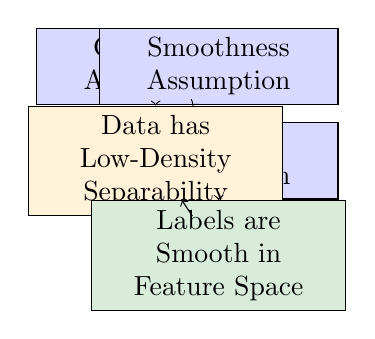
\begin{tikzpicture}[node distance=0.8cm, scale=0.7]
				\node[draw, rectangle, fill=blue!15, text width=2.8cm, align=center] (c) {Clustering\\Assumption};
				\node[draw, rectangle, fill=blue!15, text width=2.8cm, align=center] (s) [right of=c] {Smoothness\\Assumption};
				\node[draw, rectangle, fill=blue!15, text width=2.8cm, align=center] (m) [below of=s, node distance=1.2cm] {Manifold\\Assumption};
				\node[draw, rectangle, fill=orange!15, text width=3.0cm, align=center] (s2) [below of=c, node distance=1.2cm] {Data has\\Low-Density\\Separability};
				\node[draw, rectangle, fill=green!15, text width=3.0cm, align=center] (s3) [below of=m, node distance=1.2cm] {Labels are\\Smooth in\\Feature Space};
				\draw[->] (c) -- (s2);
				\draw[->] (s) -- (s2);
				\draw[->] (m) -- (s3);
				\draw[->] (s2) -- (s3);
			\end{tikzpicture}
		\end{center}
		
		\textbf{Key Connections:}
		\begin{enumerate}
			\item Clustering $\implies$ Smoothness: Clusters separated by low-density regions $\Rightarrow$ boundaries in low density
			\item Manifold $\implies$ Smoothness: If labels vary smoothly on manifold, close points on manifold have same label
			\item All $\implies$: Unlabeled data $\{x_i\}_{i=l+1}^{l+u}$ reveals structure of $P(x)$ which guides $P(y|x)$
		\end{enumerate}
		
		\textcolor{red}{\textbf{Exam Trap:}} Violation of ANY assumption can cause SSL to fail.
	\end{frame}
	
	\begin{frame}{13. When Assumptions are Satisfied - Success}
		\fontsize{6.5}{7.5}\selectfont
		\textbf{Example: Document Classification}
		
		\textbf{Data:}
		\begin{itemize}
			\item $l = 100$ labeled documents (topics: Sports, Politics, Technology)
			\item $u = 100,000$ unlabeled documents
			\item Features: TF-IDF word frequencies (high-dimensional)
		\end{itemize}
		
		\textbf{Assumptions Satisfied:}
		\begin{enumerate}
			\item \textcolor{blue}{Clustering:} Documents on same topic use similar vocabulary $\Rightarrow$ form clusters
			\item \textcolor{blue}{Smoothness:} Similar documents (cosine distance) have same topic
			\item \textcolor{blue}{Manifold:} Documents lie on topic-specific low-dimensional subspace
		\end{enumerate}
		
		\textbf{Result:}
		\begin{itemize}
			\item SSL accurately classifies unlabeled documents
			\item Outperforms supervised-only (100 labels) and unsupervised-only
			\item Unlabeled data maps topic-specific vocabulary manifolds
		\end{itemize}
		
		\textbf{Another Example: Handwritten Digit Recognition}
		\begin{itemize}
			\item 28x28 pixel images ($D=784$)
			\item 10 classes (0-9)
			\item $l = 100$ labeled digits, $u = 60,000$ unlabeled
			\item Digits of same class lie on same manifold (variations in writing style)
		\end{itemize}
	\end{frame}
	
	\begin{frame}{14. When Assumptions are Violated - Failure}
		\fontsize{6.5}{7.5}\selectfont
		\textbf{Example: Facial Recognition with Varying Pose}
		
		\textbf{Data:}
		\begin{itemize}
			\item $l = 50$ labeled face images (Person A, Person B)
			\item $u = 10,000$ unlabeled face images
			\item Features: Pixel values ($D = 10,000$)
		\end{itemize}
		
		\textbf{Problem 1 - Manifold Mixing:}
		\begin{itemize}
			\item Person A at extreme pose may look like Person B at neutral pose
			\item Same manifold may contain different people
			\item \textcolor{red}{Manifold Assumption Violated}
		\end{itemize}
		
		\textbf{Problem 2 - No Clusters:}
		\begin{itemize}
			\item Face images of different people intermingled in pixel space
			\item \textcolor{red}{Clustering Assumption Violated}
		\end{itemize}
		
		\textbf{Problem 3 - Dataset Shift:}
		\begin{itemize}
			\item Labeled images: Professional studio photos
			\item Unlabeled images: Web-crawled photos
			\item Different lighting, background, resolution
			\item \textcolor{red}{Distribution Mismatch}
		\end{itemize}
		
		\textbf{Result:}
		\begin{itemize}
			\item SSL performance degrades below supervised-only
			\item Pseudo-labels are incorrect $\Rightarrow$ error amplification
			\item \textcolor{red}{SSL is not a magic solution; assumptions matter!}
		\end{itemize}
	\end{frame}
	
	% ============================================================
	% SLIDES 15-20: INDUCTIVE VS TRANSDUCTIVE
	% ============================================================
	
	\begin{frame}{15. Inductive vs Transductive - Core Concept}
		\fontsize{6.5}{7.5}\selectfont
		\textbf{Key Distinction at Highest Level:}
		
		\begin{tabular}{|p{4.0cm}|p{5.0cm}|}
			\hline
			\textbf{Inductive} & \textbf{Transductive} \\
			\hline
			Learns a \textcolor{blue}{generalizable model} & Only labels \textcolor{blue}{current unlabeled data} \\
			\hline
			Produces function $f: X \rightarrow Y$ & No function; just assigns labels \\
			\hline
			Can classify \textcolor{blue}{new, unseen} data & Cannot handle new data \\
			\hline
			\textcolor{green}{Preferred for production/deployment} & \textcolor{orange}{Limited to offline analysis} \\
			\hline
			Examples: Self-training, Co-training & Example: Label Propagation \\
			\hline
			"Open world" view & "Closed world" view \\
			\hline
		\end{tabular}
		
		\textbf{Mathematical Formulation:}
		\begin{itemize}
			\item \textcolor{blue}{Inductive:} $\hat{f} = \arg\min_{f \in \mathcal{H}} \mathcal{L}(f, \{(x_i,y_i)\}_{i=1}^l) + \lambda \mathcal{R}(f, \{x_i\}_{i=l+1}^{l+u})$
			\item \textcolor{blue}{Transductive:} $\hat{y}_{l+1},...,\hat{y}_{l+u} = \arg\max P(y_{l+1},...,y_{l+u} | \{(x_i,y_i)\}_{i=1}^l, \{x_i\}_{i=l+1}^{l+u})$
		\end{itemize}
	\end{frame}
	
	\begin{frame}{16. Transductive Methods - Detailed}
		\fontsize{6.5}{7.5}\selectfont
		\textbf{Label Propagation (Graph-Based):}
		
		\textbf{Mathematical Framework:}
		\begin{enumerate}
			\item Build graph $G = (V,E)$ where $V = \{x_1,...,x_{l+u}\}$
			\item Edge weights $w_{ij} = \exp\left(-\frac{\|x_i - x_j\|^2}{2\sigma^2}\right)$
			\item Labels propagate through graph:
			\[
			Y^{(t+1)} = P Y^{(t)}
			\]
			where $P$ is row-normalized transition matrix
			\item Fixed point: $Y^* = \lim_{t \to \infty} Y^{(t)}$
		\end{enumerate}
		
		\textbf{Properties:}
		\begin{itemize}
			\item Labels from labeled nodes "flow" to unlabeled neighbors
			\item High confidence when surrounded by similar labeled nodes
			\item No model $f$ learned; just node labels $Y^*$
		\end{itemize}
		
		\textbf{Limitations:}
		\begin{enumerate}
			\item \textcolor{red}{No generalizable model:} Can't classify new $x_{l+u+1}$
			\item \textcolor{red}{Computational:} Graph with $n$ nodes $\Rightarrow O(n^2)$ for dense graph
			\item \textcolor{red}{Sensitive:} Choice of $\sigma$ and graph structure matters
		\end{enumerate}
		
		\textbf{When to Use:}
		\begin{itemize}
			\item Only need to label current dataset (offline analysis)
			\item No need for future predictions
			\item Small dataset where graph construction is feasible
		\end{itemize}
	\end{frame}
	
	\begin{frame}{17. Inductive Methods - Detailed}
		\fontsize{6.5}{7.5}\selectfont
		\textbf{Core Idea:}
		\begin{itemize}
			\item Learn a function $\hat{f}: \mathcal{X} \rightarrow \mathcal{Y}$ from both labeled and unlabeled data
			\item Can be applied to any new $x \notin \{x_1,...,x_{l+u}\}$
			\item \textcolor{blue}{Preferred in practice} because:
			\begin{enumerate}
				\item Deployable in production
				\item Can score new instances in real-time
				\item Adapts as new data arrives
			\end{enumerate}
		\end{itemize}
		
		\textbf{General Framework:}
		\[
		\hat{f} = \arg\min_{f \in \mathcal{H}} \underbrace{\sum_{i=1}^l \ell(f(x_i), y_i)}_{\text{Supervised Loss}} + \underbrace{\lambda_1 \sum_{i=l+1}^{l+u} \mathcal{R}(f, x_i)}_{\text{Unsupervised Regularizer}} + \underbrace{\lambda_2 \|f\|_{\mathcal{H}}^2}_{\text{Model Complexity}}
		\]
		
		\textbf{Unsupervised Regularizers:}
		\begin{enumerate}
			\item \textcolor{blue}{Low-Density Separation:} $f$ should be confident on unlabeled data
			\item \textcolor{blue}{Manifold Regularization:} $f$ should be smooth on the manifold
			\item \textcolor{blue}{Entropy Minimization:} Minimize $-\sum_{x \in \mathcal{U}} P(y|x) \log P(y|x)$
		\end{enumerate}
		
		\textbf{Main Approaches:}
		\begin{enumerate}
			\item Wrapper methods (Self-training, Co-training)
			\item Unsupervised pre-processing (PCA, Autoencoders, Cluster-then-Label)
		\end{enumerate}
	\end{frame}
	
	\begin{frame}{18. Inductive vs Transductive - Decision Framework}
		\fontsize{6.5}{7.5}\selectfont
		\textbf{Decision Matrix for Choosing:}
		
		\begin{tabular}{|p{2.8cm}|p{3.0cm}|p{3.0cm}|}
			\hline
			\textbf{Requirement} & \textbf{Inductive} & \textbf{Transductive} \\
			\hline
			Need to classify future data & \textcolor{green}{YES} & \textcolor{red}{NO} \\
			\hline
			Real-time scoring required & \textcolor{green}{YES} & \textcolor{red}{NO} \\
			\hline
			Model deployment needed & \textcolor{green}{YES} & \textcolor{red}{NO} \\
			\hline
			Only current dataset matters & \textcolor{orange}{May be overkill} & \textcolor{green}{YES} \\
			\hline
			Offline analysis only & \textcolor{orange}{Can be used} & \textcolor{green}{YES} \\
			\hline
			Computational constraints & \textcolor{orange}{More complex} & \textcolor{green}{Simpler} \\
			\hline
			Need interpretable model & \textcolor{green}{YES} & \textcolor{red}{NO} \\
			\hline
		\end{tabular}
		
		\textbf{Recommendation:}
		\begin{itemize}
			\item \textcolor{blue}{Production/Deployment:} Always use Inductive
			\item \textcolor{blue}{Research/Exploratory:} Transductive may suffice
			\item \textcolor{blue}{Risk Management:} Inductive preferred (need to score new cases)
		\end{itemize}
		
		\textcolor{red}{\textbf{Exam Trap:}} Transductive is NOT "better" or "worse"; it's "different" for different purposes.
	\end{frame}
	
	% ============================================================
	% SLIDES 19-30: SELF-TRAINING - DETAILED
	% ============================================================
	
	\begin{frame}{19. Self-Training - Algorithm Overview}
		\fontsize{6.5}{7.5}\selectfont
		\textbf{Definition:}
		\begin{itemize}
			\item "Wrapper" method using supervised classifier iteratively
			\item Also called \textcolor{blue}{"Pseudo-labeling"} or \textcolor{blue}{"Bootstrapping"}
			\item Uses unlabeled data from a supervised perspective
		\end{itemize}
		
		\textbf{Full Algorithm:}
		
		\begin{enumerate}
			\item Train classifier $f$ on labeled set $\mathcal{L} = \{(x_i, y_i)\}_{i=1}^l$
			\item Apply $f$ to all unlabeled set $\mathcal{U} = \{x_i\}_{i=l+1}^{l+u}$
			\item Obtain predicted labels $\hat{y}_i = f(x_i)$ and confidence scores $p_i = P(\hat{y}_i | x_i)$
			\item Select most confident prediction: $j = \arg\max_{i \in \mathcal{U}} p_i$
			\item Move $(x_j, \hat{y}_j)$ from $\mathcal{U}$ to $\mathcal{L}$
			\item Repeat from Step 1 until $\mathcal{U} = \emptyset$ or stopping criterion
		\end{enumerate}
		
		\textbf{Pseudo-label Formalism:}
		\[
		\hat{y}_i = \arg\max_{c \in \{1,...,C\}} f_c(x_i), \quad \text{with confidence } \max_c f_c(x_i)
		\]
		
		\textbf{Stopping Criteria:}
		\begin{itemize}
			\item All unlabeled instances labeled
			\item Confidence below threshold $\theta$
			\item Maximum iterations reached
			\item Validation performance plateaus/degrades
		\end{itemize}
	\end{frame}
	
	\begin{frame}{20. Self-Training - Mathematical Framework}
		\fontsize{6.5}{7.5}\selectfont
		\textbf{Objective Function:}
		\[
		\min_f \sum_{i=1}^l \ell(f(x_i), y_i) + \lambda \sum_{i=l+1}^{l+u} \ell(f(x_i), \hat{y}_i)
		\]
		where $\hat{y}_i$ are pseudo-labels (dependent on $f$)
		
		\textbf{Iterative Optimization:}
		
		At iteration $t$:
		\[
		f^{(t)} = \arg\min_f \sum_{i=1}^{l + m_t} \ell(f(x_i), y_i^{(t)})
		\]
		where $y_i^{(t)}$ are:
		\begin{itemize}
			\item Original labels for $i \leq l$
			\item Pseudo-labels from iteration $t-1$ for $l < i \leq l + m_t$
		\end{itemize}
		
		\textbf{Confidence Selection:}
		\[
		(x_j, \hat{y}_j) = \arg\max_{i \in \mathcal{U}} f_{i, \max}^{(t)}(x_i)
		\]
		where $f_{i,\max}(x_i) = \max_c f_c(x_i)$
		
		\textbf{Batch Selection (k instances):}
		\[
		\{(x_j, \hat{y}_j)\}_{j=1}^k = \text{top-}k \text{ instances by } f_{i,\max}(x_i)
		\]
		Reduces computational cost by $k$ times.
	\end{frame}
	
	\begin{frame}{21. Self-Training - Advantages}
		\fontsize{6.5}{7.5}\selectfont
		\textbf{Key Strengths:}
		
		\begin{enumerate}
			\item \textcolor{blue}{Algorithm Agnostic:}
			\begin{itemize}
				\item Works with ANY supervised classifier: Logistic Regression, SVM, Decision Trees, Neural Networks
				\item No modification to base classifier needed
				\item Only requires confidence scores (probabilities)
			\end{itemize}
			
			\item \textcolor{blue}{Simplicity:}
			\begin{itemize}
				\item Intuitive and easy to implement
				\item Minimal hyperparameters
				\item Clear iterative process
			\end{itemize}
			
			\item \textcolor{blue}{Flexibility:}
			\begin{itemize}
				\item Can be applied to classification and regression
				\item Can handle multi-class problems
				\item Can be combined with other techniques
			\end{itemize}
			
			\item \textcolor{blue}{Scalability:}
			\begin{itemize}
				\item Batch processing (add $k$ instances at a time)
				\item Can handle large datasets with efficient classifiers
				\item Parallelizable (train multiple models in parallel)
			\end{itemize}
			
			\item \textcolor{blue}{No Feature Split Required:}
			\begin{itemize}
				\item Unlike co-training, doesn't need two views
				\item Can be applied to any feature set
			\end{itemize}
		\end{enumerate}
	\end{frame}
	
	\begin{frame}{22. Self-Training - Disadvantages \& Risks}
		\fontsize{6.5}{7.5}\selectfont
		\textbf{Major Risks:}
		
		\begin{enumerate}
			\item \textcolor{red}{Error Amplification:}
			\begin{itemize}
				\item Initial mistakes with high confidence are added to training set
				\item These errors propagate and reinforce in subsequent iterations
				\item Self-reinforcing feedback loop
				\item \textcolor{red}{Example:} Model misclassifies a fraud case as normal with 99\% confidence, then learns from this error
			\end{itemize}
			
			\item \textcolor{red}{Computational Cost:}
			\begin{itemize}
				\item Model retrained each iteration
				\item If adding 1 instance at a time: $u$ retraining steps
				\item Batch method: $u/k$ retraining steps (mitigation)
			\end{itemize}
			
			\item \textcolor{red}{Overfitting:}
			\begin{itemize}
				\item Model learns its own noise and biases
				\item Validation performance degrades after early iterations
				\item Memorizes pseudo-labels rather than generalizing
			\end{itemize}
			
			\item \textcolor{red}{Class Imbalance Amplification:}
			\begin{itemize}
				\item Model biased toward majority class
				\item High-confidence predictions from majority class
				\item Amplifies imbalance over iterations
			\end{itemize}
		\end{enumerate}
	\end{frame}
	
	\begin{frame}{23. Self-Training - Mitigation Strategies}
		\fontsize{6.5}{7.5}\selectfont
		\textbf{Addressing Error Amplification:}
		
		\begin{enumerate}
			\item \textcolor{blue}{Confidence Threshold:}
			\begin{itemize}
				\item Only add predictions with confidence $> \theta$
				\item Typical: $\theta = 0.9$ or $0.95$
				\item \textcolor{red}{Trade-off:} Too high $\Rightarrow$ few labels added; too low $\Rightarrow$ errors introduced
			\end{itemize}
			
			\item \textcolor{blue}{Batch Processing:}
			\begin{itemize}
				\item Add $k$ most confident instances per iteration
				\item Reduces computational cost by factor $k$
				\item Still risk of adding multiple erroneous labels
			\end{itemize}
			
			\item \textcolor{blue}{Validation Set:}
			\begin{itemize}
				\item Monitor performance on held-out validation set
				\item Stop when performance degrades
				\item Ensures model doesn't overfit to pseudo-labels
			\end{itemize}
			
			\item \textcolor{blue}{Co-Training:}
			\begin{itemize}
				\item Use two models with different views
				\item Cross-teaching reduces error amplification
				\item \textcolor{blue}{See Section on Co-training}
			\end{itemize}
			
			\item \textcolor{blue}{Ensemble Methods:}
			\begin{itemize}
				\item Use multiple models and only add when all agree
				\item Reduces risk of individual model errors
			\end{itemize}
		\end{enumerate}
	\end{frame}
	
	\begin{frame}{24. Self-Training - Worked Example (Borrowers)}
		\fontsize{6.5}{7.5}\selectfont
		\textbf{Dataset:} 14 borrowers, 10 labeled, 4 unlabeled
		
		\textbf{Features:} Balance (Feature A), Income (Feature B)
		
		\textbf{Classifier:} Logistic Regression
		
		\textbf{Step 1:} Train on labeled (1-10):
		\[
		P(\text{Default}) = \frac{1}{1 + e^{-(\beta_0 + \beta_1 \text{Balance} + \beta_2 \text{Income})}}
		\]
		
		\textbf{Step 2:} Predict unlabeled (11-14):
		
		\begin{tabular}{|c|c|c|c|}
			\hline
			Borrower & $P(\text{Non-Default})$ & $P(\text{Default})$ & Prediction \\
			\hline
			11 & 1.0000 & $8.08 \times 10^{-29}$ & 0 (Non-Default) \\
			12 & 0.9934 & $6.61 \times 10^{-3}$ & 0 \\
			13 & 0.0000 & 1.0000 & 1 (Default) \\
			14 & 0.9896 & $1.04 \times 10^{-2}$ & 0 \\
			\hline
		\end{tabular}
		
		\textbf{Step 3:} Add Borrower 13 (highest confidence: $P=1.000$) to labeled set
		
		\textbf{Iterate:} Retrain, predict remaining, add next most confident
		
		\textbf{Final Labels:} 11, 12, 14 $\rightarrow$ Non-Default; 13 $\rightarrow$ Default
		
		\textcolor{red}{\textbf{Key Insight:}} Near-perfect probabilities suggest overfitting on small sample.
	\end{frame}
	
	\begin{frame}{25. Self-Training - Mathematical Example Details}
		\fontsize{6.5}{7.5}\selectfont
		\textbf{Logistic Regression Setup:}
		
		Initial model (first iteration):
		\[
		\log\left(\frac{P}{1-P}\right) = \beta_0 + \beta_1 \text{Balance} + \beta_2 \text{Income}
		\]
		
		\textbf{Prediction for Borrower 13:}
		\begin{itemize}
			\item Balance = 1.99, Income = -1.04
			\item $\beta_0 + \beta_1(1.99) + \beta_2(-1.04) \approx 20.3$
			\item $P(\text{Default}) = \frac{1}{1 + e^{-20.3}} = 1.0000$
		\end{itemize}
		
		\textbf{Why such high confidence?}
		\begin{itemize}
			\item Small labeled set (n=10)
			\item Features are highly predictive in this limited sample
			\item Model overfits to patterns in the labeled data
			\item \textcolor{red}{Risk:} If Borrower 13 is actually Non-Default, error is severe
		\end{itemize}
		
		\textbf{After Adding Borrower 13:}
		
		New model includes Borrower 13 (labeled Default):
		\begin{itemize}
			\item Decision boundary shifts toward Default class
			\item Borrower 11 now most confident Non-Default
			\item Pattern: Model reinforces initial high-confidence predictions
		\end{itemize}
		
		\textcolor{red}{\textbf{Exam Trap:}} High confidence $\neq$ correct label. Overfitting causes overconfidence.
	\end{frame}
	
	% ============================================================
	% SLIDES 26-36: CO-TRAINING - DETAILED
	% ============================================================
	
	\begin{frame}{26. Co-Training - Algorithm Overview}
		\fontsize{6.5}{7.5}\selectfont
		\textbf{Definition:}
		\begin{itemize}
			\item Inductive method using \textcolor{blue}{two different "views"} of the data
			\item Two classifiers "teach" each other
			\item Reduces risk of error amplification (self-training weakness)
		\end{itemize}
		
		\textbf{Key Requirement:}
		\begin{itemize}
			\item Features can be split into \textcolor{blue}{two disjoint and conditionally independent} subsets
			\item Each view should be sufficient to build a good classifier on its own
			\item Views are conditionally independent given the class label
		\end{itemize}
		
		\textbf{Algorithm:}
		\begin{enumerate}
			\item Split features into Group A and Group B
			\item Train Model A on Group A (labeled data), Model B on Group B (labeled data)
			\item Model A predicts labels for all unlabeled using Group A
			\item Model B predicts labels for all unlabeled using Group B
			\item Select most confident prediction from Model A $\rightarrow$ add to Model B's training set
			\item Select most confident prediction from Model B $\rightarrow$ add to Model A's training set
			\item Retrain both models, repeat until no unlabeled data remains
		\end{enumerate}
	\end{frame}
	
	\begin{frame}{27. Co-Training - Mathematical Framework}
		\fontsize{6.5}{7.5}\selectfont
		\textbf{Conditional Independence Assumption:}
		\[
		P(x_A, x_B | y) = P(x_A | y) \cdot P(x_B | y)
		\]
		where $x_A$ and $x_B$ are the two feature views.
		
		\textbf{Two Classifiers:}
		\[
		f_A: \mathcal{X}_A \rightarrow \mathcal{Y}, \quad f_B: \mathcal{X}_B \rightarrow \mathcal{Y}
		\]
		
		\textbf{Cross-Teaching Objective:}
		At iteration $t$:
		\[
		f_A^{(t)} = \arg\min_{f_A} \sum_{i=1}^{l + m_t^{(A)}} \ell(f_A(x_{i,A}), y_i)
		\]
		\[
		f_B^{(t)} = \arg\min_{f_B} \sum_{i=1}^{l + m_t^{(B)}} \ell(f_B(x_{i,B}), y_i)
		\]
		where $m_t^{(A)}$ and $m_t^{(B)}$ are pseudo-labels added from the other model.
		
		\textbf{Confidence Selection:}
		\[
		(x_j, \hat{y}_j) = \arg\max_{i \in \mathcal{U}} \max_c f_{A,c}(x_{i,A}) \quad \text{(for Model A's most confident)}
		\]
		\[
		(x_k, \hat{y}_k) = \arg\max_{i \in \mathcal{U}} \max_c f_{B,c}(x_{i,B}) \quad \text{(for Model B's most confident)}
		\]
	\end{frame}
	
	\begin{frame}{28. Co-Training - Theoretical Justification}
		\fontsize{6.5}{7.5}\selectfont
		\textbf{Why Co-Training Works (Theory):}
		
		\textbf{Theorem (Blum \& Mitchell, 1998):}
		\begin{itemize}
			\item If features are conditionally independent given the class
			\item AND each view is sufficient for learning
			\item THEN co-training can learn from unlabeled data
			\item The two views provide "independent evidence" for labels
		\end{itemize}
		
		\textbf{Intuitive Explanation:}
		\begin{itemize}
			\item Model A makes mistakes on some instances
			\item Model B makes mistakes on different instances
			\item When both confidently agree, probability of error is product of individual error probabilities
			\item Since views are independent: $P(\text{both wrong}) = P(A\text{ wrong}) \cdot P(B\text{ wrong})$
			\item If each is 90\% accurate: $P(\text{both wrong}) = 0.1 \times 0.1 = 0.01$
		\end{itemize}
		
		\textbf{Error Amplification Reduction:}
		\begin{itemize}
			\item Self-training: Model learns from its own errors $\Rightarrow$ amplification
			\item Co-training: Model learns from other model's evidence $\Rightarrow$ correction
			\item Mistakes are "filtered" through the other view
		\end{itemize}
	\end{frame}
	
	\begin{frame}{29. Co-Training - Advantages \& Disadvantages}
		\fontsize{6.5}{7.5}\selectfont
		\textbf{Advantages:}
		
		\begin{enumerate}
			\item \textcolor{blue}{Reduced Error Amplification:}
			\begin{itemize}
				\item Cross-teaching prevents self-reinforcing errors
				\item Each model's mistakes are corrected by the other
			\end{itemize}
			
			\item \textcolor{blue}{Leverages Multiple Views:}
			\begin{itemize}
				\item Can combine different feature types (text + metadata)
				\item Uses complementary information from both views
			\end{itemize}
			
			\item \textcolor{blue}{Robustness:}
			\begin{itemize}
				\item More robust than self-training
				\item Less sensitive to initial model errors
			\end{itemize}
		\end{enumerate}
		
		\textbf{Disadvantages:}
		
		\begin{enumerate}
			\item \textcolor{red}{Requires Feature Split:}
			\begin{itemize}
				\item Must find two independent views
				\item Not always possible in practice
			\end{itemize}
			
			\item \textcolor{red}{Conditional Independence:}
			\begin{itemize}
				\item Strong assumption
				\item Often violated in real data
			\end{itemize}
			
			\item \textcolor{red}{Computational Cost:}
			\begin{itemize}
				\item Two models $\Rightarrow$ double the cost
				\item Still iterative like self-training
			\end{itemize}
		\end{enumerate}
	\end{frame}
	
	\begin{frame}{30. Co-Training - Worked Example (Borrowers)}
		\fontsize{6.5}{7.5}\selectfont
		\textbf{Feature Split:}
		\begin{itemize}
			\item Group A: Balance (Feature A)
			\item Group B: Income (Feature B)
		\end{itemize}
		
		\textbf{Step 1:} Train Model A (Balance), Model B (Income)
		
		\textbf{Model A Predictions:}
		
		\begin{tabular}{|c|c|c|c|}
			\hline
			Borrower & $P(\text{Non-Default})$ & $P(\text{Default})$ & Prediction \\
			\hline
			11 & 1.0000 & $1.32 \times 10^{-30}$ & 0 \\
			12 & 0.9991 & $9.13 \times 10^{-4}$ & 0 \\
			13 & 0.0000 & 1.0000 & 1 \\
			14 & 0.9983 & $1.74 \times 10^{-2}$ & 0 \\
			\hline
		\end{tabular}
		
		\textbf{Model B Predictions:}
		
		\begin{tabular}{|c|c|c|c|}
			\hline
			Borrower & $P(\text{Non-Default})$ & $P(\text{Default})$ & Prediction \\
			\hline
			11 & 0.9989 & $1.14 \times 10^{-3}$ & 0 \\
			12 & 0.9635 & $3.65 \times 10^{-2}$ & 0 \\
			13 & 0.1655 & 0.8346 & 1 \\
			14 & 0.9507 & $4.93 \times 10^{-2}$ & 0 \\
			\hline
		\end{tabular}
		
		\textbf{Cross-Teaching:}
		\begin{itemize}
			\item Model A most confident: Borrower 13 (Default) $\rightarrow$ add to Model B's training set
			\item Model B most confident: Borrower 11 (Non-Default) $\rightarrow$ add to Model A's training set
		\end{itemize}
	\end{frame}
	
	\begin{frame}{31. Co-Training - Feature Split Requirements}
		\fontsize{6.5}{7.5}\selectfont
		\textbf{Condition 1: Disjoint Features}
		\[
		\text{Feature Set } \mathcal{F} = \mathcal{F}_A \cup \mathcal{F}_B, \quad \mathcal{F}_A \cap \mathcal{F}_B = \emptyset
		\]
		
		\textbf{Condition 2: Conditional Independence}
		\[
		P(x_A, x_B | y) = P(x_A | y) \cdot P(x_B | y)
		\]
		
		\textbf{Condition 3: Sufficiency}
		\begin{itemize}
			\item Each view alone can build a reasonably good classifier
			\item $P(y|x_A)$ is informative (not random)
			\item $P(y|x_B)$ is informative (not random)
		\end{itemize}
		
		\textbf{Examples of Good Splits:}
		
		\begin{tabular}{|p{3.0cm}|p{3.0cm}|p{3.0cm}|}
			\hline
			\textbf{Domain} & \textbf{View A} & \textbf{View B} \\
			\hline
			Web Pages & Words on page & Anchor text from links \\
			\hline
			Emails & Subject line words & Body text words \\
			\hline
			Images & RGB pixels & Edge/HOG features \\
			\hline
			Video & Audio track & Video frames \\
			\hline
			Documents & TF-IDF words & Meta-data (author, date) \\
			\hline
			Medical & Clinical notes & Lab results \\
			\hline
		\end{tabular}
	\end{frame}
	
	\begin{frame}{32. Co-Training - When It Fails}
		\fontsize{6.5}{7.5}\selectfont
		\textbf{Reason 1: Views Not Conditionally Independent}
		\begin{itemize}
			\item Example: Web page classification where content and anchor text are correlated
			\item Author writes about same topics in text and links
			\item \textcolor{red}{Result:} Models make same errors, no correction
		\end{itemize}
		
		\textbf{Reason 2: Views Not Sufficient}
		\begin{itemize}
			\item Example: One view has very weak predictive power
			\item Model B (weak view) makes mostly random predictions
			\item \textcolor{red}{Result:} Adds noisy labels to Model A, degrades performance
		\end{itemize}
		
		\textbf{Reason 3: No Natural Feature Split}
		\begin{itemize}
			\item Many datasets have highly correlated features
			\item Example: Financial ratios (all based on accounting data)
			\item \textcolor{red}{Result:} Cannot find two independent views
		\end{itemize}
		
		\textbf{Reason 4: Dataset Shift}
		\begin{itemize}
			\item Labeled data distribution differs from unlabeled
			\item Models learn wrong structure from unlabeled
			\item \textcolor{red}{Result:} Co-training fails worse than self-training
		\end{itemize}
	\end{frame}
	
	% ============================================================
	% SLIDES 33-40: UNSUPERVISED PRE-PROCESSING
	% ============================================================
	
	\begin{frame}{33. Unsupervised Pre-Processing - Overview}
		\fontsize{6.5}{7.5}\selectfont
		\textbf{Definition:}
		\begin{itemize}
			\item Use unlabeled data \textcolor{blue}{first}, before supervised learning
			\item Learn about data structure or create efficient feature representation
			\item Three main strategies:
			\begin{enumerate}
				\item Feature Extraction (PCA, Autoencoders)
				\item Cluster-then-Label
				\item Pre-training (Deep Learning)
			\end{enumerate}
		\end{itemize}
		
		\textbf{Core Philosophy:}
		\begin{itemize}
			\item Unlabeled data is used to improve \textcolor{blue}{representation}
			\item Supervised learning uses this improved representation
			\item Two-stage process: Unsupervised $\rightarrow$ Supervised
		\end{itemize}
		
		\textbf{When to Use:}
		\begin{itemize}
			\item When unlabeled data is abundant
			\item When features are high-dimensional or noisy
			\item When representation learning is critical
			\item When deep learning is involved (pre-training)
		\end{itemize}
	\end{frame}
	
	\begin{frame}{34. Feature Extraction - PCA}
		\fontsize{6.5}{7.5}\selectfont
		\textbf{Principal Component Analysis (PCA):}
		
		\textbf{Mathematical Formulation:}
		\[
		X = U\Sigma V^T \quad \text{(SVD Decomposition)}
		\]
		\[
		X_{\text{PCA}} = X V_k \quad \text{where } V_k \text{ top } k \text{ eigenvectors}
		\]
		
		\textbf{Process:}
		\begin{enumerate}
			\item Compute covariance matrix: $\Sigma = \frac{1}{n} X^T X$
			\item Find eigenvectors $v_1, ..., v_D$ with eigenvalues $\lambda_1 \geq \lambda_2 \geq ... \geq \lambda_D$
			\item Select top $k$ eigenvectors: $V_k = [v_1, ..., v_k]$
			\item Project data: $Z = X V_k$ (reduced dimensions)
			\item Train supervised classifier on $Z$ using labeled data
		\end{enumerate}
		
		\textbf{Advantages:}
		\begin{itemize}
			\item Reduces dimensionality (helps with overfitting)
			\item Captures maximum variance in data
			\item Unsupervised (doesn't use labels)
		\end{itemize}
		
		\textbf{Disadvantages:}
		\begin{itemize}
			\item \textcolor{red}{Linear:} Cannot capture non-linear structure
			\item \textcolor{red}{Variance-focused:} May discard discriminative features with low variance
		\end{itemize}
	\end{frame}
	
	\begin{frame}{35. Feature Extraction - Autoencoders}
		\fontsize{6.5}{7.5}\selectfont
		\textbf{Autoencoder Architecture:}
		\[
		h = \sigma_e(W_e x + b_e) \quad \text{(Encoder)}
		\]
		\[
		\hat{x} = \sigma_d(W_d h + b_d) \quad \text{(Decoder)}
		\]
		
		\textbf{Objective:} Minimize reconstruction error:
		\[
		\mathcal{L}_{\text{AE}} = \|x - \hat{x}\|^2 = \|x - \sigma_d(W_d \sigma_e(W_e x + b_e) + b_d)\|^2
		\]
		
		\textbf{Process:}
		\begin{enumerate}
			\item Train autoencoder on ALL data (labeled + unlabeled)
			\item Encoder learns compressed representation $h$ for each $x$
			\item $h$ captures essential features in lower dimension ($d \ll D$)
			\item Use $h$ as features for supervised classifier on labeled data
		\end{enumerate}
		
		\textbf{Advantages over PCA:}
		\begin{itemize}
			\item \textcolor{blue}{Non-linear:} Can capture complex structure
			\item \textcolor{blue}{Flexible:} Can be deeper, more expressive
			\item \textcolor{blue}{Learns features:} Not just variance, but reconstruction
		\end{itemize}
		
		\textbf{Disadvantages:}
		\begin{itemize}
			\item \textcolor{red}{Computational:} More expensive than PCA
			\item \textcolor{red}{Hyperparameter Tuning:} Architecture, learning rate, etc.
		\end{itemize}
	\end{frame}
	
	\begin{frame}{36. Cluster-then-Label - Detailed}
		\fontsize{6.5}{7.5}\selectfont
		\textbf{Two-Stage Process:}
		
		\textbf{Stage 1: Clustering (Unsupervised)}
		\begin{itemize}
			\item Apply clustering algorithm (e.g., K-means) to ALL data
			\item Partition data into $k$ clusters: $\mathcal{C}_1, ..., \mathcal{C}_k$
			\item Based on feature similarity, NOT labels
		\end{itemize}
		
		\textbf{K-means Objective:}
		\[
		\min_{\mu_1,...,\mu_k} \sum_{j=1}^k \sum_{x_i \in \mathcal{C}_j} \|x_i - \mu_j\|^2
		\]
		
		\textbf{Stage 2: Label Assignment}
		\begin{itemize}
			\item For each cluster $\mathcal{C}_j$, find labeled points $\mathcal{L}_j \subset \mathcal{C}_j$
			\item Assign cluster label: $\hat{y}_j = \text{majority}(\{y_i : i \in \mathcal{L}_j\})$
			\item If no labels in cluster: unassigned (or nearest cluster)
			\item All unlabeled points in cluster get $\hat{y}_j$
		\end{itemize}
		
		\textbf{Final Step:}
		\begin{itemize}
			\item Train supervised classifier on fully labeled dataset
			\item Pseudo-labels become training data
		\end{itemize}
		
		\textbf{Limitation:}
		\begin{itemize}
			\item \textcolor{red}{Relies on Clustering Assumption}
			\item If clusters don't correspond to classes, all pseudo-labels wrong
		\end{itemize}
	\end{frame}
	
	\begin{frame}{37. Cluster-then-Label - Advantages \& Risks}
		\fontsize{6.5}{7.5}\selectfont
		\textbf{Advantages:}
		
		\begin{enumerate}
			\item \textcolor{blue}{Computational Efficiency:}
			\begin{itemize}
				\item Single clustering pass (O(nkd) iterations)
				\item No iterative model retraining
				\item Much faster than self-training/co-training
			\end{itemize}
			
			\item \textcolor{blue}{Simplicity:}
			\begin{itemize}
				\item Easy to understand and implement
				\item Few hyperparameters (k, distance metric)
			\end{itemize}
			
			\item \textcolor{blue}{Scalable:}
			\begin{itemize}
				\item Works with large datasets
				\item K-means scales O(n) with efficient implementations
			\end{itemize}
		\end{enumerate}
		
		\textbf{Risks:}
		
		\begin{enumerate}
			\item \textcolor{red}{Assumption Dependency:}
			\begin{itemize}
				\item Requires Clustering Assumption to be strongly satisfied
				\item If violated, method fails completely
			\end{itemize}
			
			\item \textcolor{red}{Propagation of Errors:}
			\begin{itemize}
				\item One mislabeled cluster affects all points in it
				\item No mechanism to correct mistakes
			\end{itemize}
			
			\item \textcolor{red}{Choice of k:}
			\begin{itemize}
				\item Must know number of clusters (classes)
				\item Wrong k leads to poor results
			\end{itemize}
		\end{enumerate}
	\end{frame}
	
	\begin{frame}{38. Pre-training (Deep Learning)}
		\fontsize{6.5}{7.5}\selectfont
		\textbf{Definition:}
		\begin{itemize}
			\item Use unlabeled data to \textcolor{blue}{initialize} neural network weights
			\item Two-phase approach: Pre-training + Fine-tuning
		\end{itemize}
		
		\textbf{Phase 1: Unsupervised Pre-training}
		\begin{itemize}
			\item Train autoencoder or generative model on unlabeled data
			\item Objective: Learn good feature representations
			\item Output: Initialized weights for neural network
		\end{itemize}
		
		\textbf{Phase 2: Supervised Fine-tuning}
		\begin{itemize}
			\item Use labeled data to fine-tune the network
			\item Adjust weights for classification task
			\item Typically uses smaller learning rate
		\end{itemize}
		
		\textbf{Mathematical Framework:}
		
		Pre-training:
		\[
		\theta_{\text{pre}} = \arg\min_\theta \sum_{i=l+1}^{l+u} \|x_i - \hat{x}_i(x_i; \theta)\|^2
		\]
		
		Fine-tuning:
		\[
		\theta_{\text{final}} = \arg\min_\theta \sum_{i=1}^l \ell(f(x_i; \theta), y_i) + \lambda \|\theta - \theta_{\text{pre}}\|^2
		\]
		
		\textbf{Key Insight:} Pre-training gives model a "head start" in understanding data structure.
	\end{frame}
	
	\begin{frame}{39. Pre-training - Benefits \& Limitations}
		\fontsize{6.5}{7.5}\selectfont
		\textbf{Benefits:}
		
		\begin{enumerate}
			\item \textcolor{blue}{Better Generalization:}
			\begin{itemize}
				\item Pre-training acts as regularization
				\item Reduces overfitting with limited labels
			\end{itemize}
			
			\item \textcolor{blue}{Faster Convergence:}
			\begin{itemize}
				\item Starts from good initial weights
				\item Fine-tuning requires fewer iterations
			\end{itemize}
			
			\item \textcolor{blue}{Leverages Unlabeled Data:}
			\begin{itemize}
				\item Massive unlabeled datasets can be used
				\item Learns rich feature representations
			\end{itemize}
			
			\item \textcolor{blue}{State-of-the-art:}
			\begin{itemize}
				\item Used in modern deep learning (BERT, GPT, etc.)
				\item Essential for low-label scenarios
			\end{itemize}
		\end{enumerate}
		
		\textbf{Limitations:}
		
		\begin{enumerate}
			\item \textcolor{red}{Computational Cost:}
			\begin{itemize}
				\item Pre-training on large datasets is expensive
				\item Requires significant GPU resources
			\end{itemize}
			
			\item \textcolor{red}{Architecture Design:}
			\begin{itemize}
				\item Autoencoder must be designed carefully
				\item Too simple $\Rightarrow$ poor representation
				\item Too complex $\Rightarrow$ overfitting
			\end{itemize}
			
			\item \textcolor{red}{Transfer Mismatch:}
			\begin{itemize}
				\item Pre-training distribution may differ from task
				\item Fine-tuning may not overcome mismatch
			\end{itemize}
		\end{enumerate}
	\end{frame}
	
	\begin{frame}{40. Comparison of Pre-Processing Methods}
		\fontsize{6.5}{7.5}\selectfont
		\textbf{Comparison Table:}
		
		\begin{tabular}{|p{2.2cm}|p{2.2cm}|p{2.2cm}|p{2.2cm}|}
			\hline
			\textbf{Aspect} & \textbf{PCA} & \textbf{Autoencoder} & \textbf{Cluster-then-Label} \\
			\hline
			Type & Linear & Non-linear & Two-stage \\
			\hline
			Use of Unlabeled & All data & All data & All data \\
			\hline
			Output & Low-dim features & Low-dim features & Pseudo-labels \\
			\hline
			Computational Cost & Low & Medium-High & Low \\
			\hline
			Assumptions & Linear structure & Architecture design & Clustering \\
			\hline
			Scalability & Good & Moderate & Good \\
			\hline
			Interpretability & High & Low & Medium \\
			\hline
			Risk & Discards info & Overfitting & Assumption violation \\
			\hline
		\end{tabular}
		
		\textbf{When to Use Each:}
		\begin{itemize}
			\item \textcolor{blue}{PCA:} Linear data, need speed and interpretability
			\item \textcolor{blue}{Autoencoder:} Non-linear data, deep learning pipeline
			\item \textcolor{blue}{Cluster-then-Label:} Strong clustering, computationally efficient
		\end{itemize}
	\end{frame}
	
	% ============================================================
	% SLIDES 41-48: EXAM TRAPS AND COMMON MISCONCEPTIONS
	% ============================================================
	
	\begin{frame}{41. Exam Trap 1: Assumptions are Optional}
		\fontsize{6.5}{7.5}\selectfont
		\textbf{The Misconception:}
		\begin{itemize}
			\item "Semi-supervised learning always improves performance because it uses more data"
			\item "The assumptions are just theoretical, they don't matter in practice"
		\end{itemize}
		
		\textbf{The Reality:}
		\begin{itemize}
			\item \textcolor{red}{FALSE!} SSL only works if assumptions are satisfied
			\item If assumptions violated, SSL can perform \textcolor{red}{worse} than supervised-only
		\end{itemize}
		
		\textbf{Example:}
		\begin{itemize}
			\item Supervised-only with 100 labels: 70\% accuracy
			\item SSL with 100 labels + 10,000 unlabeled: 55\% accuracy
			\item Why? Unlabeled data misleads the model
		\end{itemize}
		
		\textbf{Key Takeaway:}
		\begin{itemize}
			\item Always check assumptions before applying SSL
			\item Test with small experiments before full deployment
			\item Monitor performance degradation as iterations progress
		\end{itemize}
		
		\textcolor{blue}{\textbf{Exam Expectation:}} You must know that SSL requires assumptions and can fail.
	\end{frame}
	
	\begin{frame}{42. Exam Trap 2: Transductive vs Inductive Confusion}
		\fontsize{6.5}{7.5}\selectfont
		\textbf{The Misconception:}
		\begin{itemize}
			\item "Transductive methods are just a type of inductive method"
			\item "Both create models that can predict new data"
		\end{itemize}
		
		\textbf{The Reality:}
		\begin{itemize}
			\item \textcolor{red}{FALSE!} They are fundamentally different
			\item Transductive $\neq$ Inductive
		\end{itemize}
		
		\textbf{Key Differences to Remember:}
		
		\begin{tabular}{|p{3.5cm}|p{3.5cm}|}
			\hline
			\textbf{Transductive} & \textbf{Inductive} \\
			\hline
			No model created & Model created \\
			\hline
			Only current data & Generalizes to new data \\
			\hline
			Cannot deploy & Deployable \\
			\hline
			Offline analysis & Production-ready \\
			\hline
		\end{tabular}
		
		\textbf{Example:}
		\begin{itemize}
			\item Label Propagation: Transductive (no model)
			\item Self-training: Inductive (creates model)
		\end{itemize}
		
		\textcolor{blue}{\textbf{Exam Expectation:}} You must be able to classify methods correctly and choose appropriate for scenario.
	\end{frame}
	
	\begin{frame}{43. Exam Trap 3: High Confidence = Correct}
		\fontsize{6.5}{7.5}\selectfont
		\textbf{The Misconception:}
		\begin{itemize}
			\item "If the model is 99\% confident, the prediction must be correct"
			\item "High confidence pseudo-labels are always reliable"
		\end{itemize}
		
		\textbf{The Reality:}
		\begin{itemize}
			\item \textcolor{red}{FALSE!} Confidence  not equal Correctness
			\item Overconfident models make mistakes with high confidence
		\end{itemize}
		
		\textbf{Why This Happens:}
		\begin{enumerate}
			\item \textcolor{blue}{Small Labeled Set:} Model overfits to few examples
			\item \textcolor{blue}{Class Imbalance:} Model is confident about majority class
			\item \textcolor{blue}{Noisy Features:} Spurious correlations in labeled data
		\end{enumerate}
		
		\textbf{Example (Borrowers):}
		\begin{itemize}
			\item Borrower 13 predicted Default with $P=1.0000$
			\item This was based on only 10 labeled examples
			\item If label was wrong, error would be severe
		\end{itemize}
		
		\textbf{Prevention:}
		\begin{itemize}
			\item Use validation set to monitor confidence calibration
			\item Use confidence thresholds
			\item Consider ensemble methods
		\end{itemize}
	\end{frame}
	
	\begin{frame}{44. Exam Trap 4: Error Amplification}
		\fontsize{6.5}{7.5}\selectfont
		\textbf{The Misconception:}
		\begin{itemize}
			\item "Adding pseudo-labels always helps because it adds more training data"
			\item "Self-training will eventually converge to the correct labels"
		\end{itemize}
		
		\textbf{The Reality:}
		\begin{itemize}
			\item \textcolor{red}{FALSE!} Self-training amplifies errors
			\item Once an error is introduced, it reinforces itself
		\end{itemize}
		
		\textbf{The Amplification Cycle:}
		
		\begin{center}
			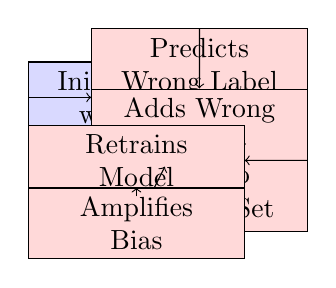
\begin{tikzpicture}[scale=0.6, node distance=0.8cm]
				\node[draw, rectangle, fill=blue!15, text width=2.5cm, align=center] (a) {Initial Model\\with Bias};
				\node[draw, rectangle, fill=red!15, text width=2.5cm, align=center] (b) [right of=a] {Predicts\\Wrong Label\\with High Confidence};
				\node[draw, rectangle, fill=red!15, text width=2.5cm, align=center] (c) [below of=b] {Adds Wrong\\Pseudo-Label to\\Training Set};
				\node[draw, rectangle, fill=red!15, text width=2.5cm, align=center] (d) [left of=c] {Retrains\\Model};
				\node[draw, rectangle, fill=red!15, text width=2.5cm, align=center] (e) [below of=d] {Amplifies\\Bias};
				\draw[->] (a) -- (b);
				\draw[->] (b) -- (c);
				\draw[->] (c) -- (d);
				\draw[->] (d) -- (e);
				\draw[->] (e) -- (b);
			\end{tikzpicture}
		\end{center}
		
		\textbf{Solution:}
		\begin{itemize}
			\item Co-training (cross-teaching)
			\item Confidence thresholds
			\item Ensemble methods
		\end{itemize}
	\end{frame}
	
	\begin{frame}{45. Exam Trap 5: More Data Always Better}
		\fontsize{6.5}{7.5}\selectfont
		\textbf{The Misconception:}
		\begin{itemize}
			\item "More data is always better for machine learning"
			\item "Unlabeled data can only help, never hurt"
		\end{itemize}
		
		\textbf{The Reality:}
		\begin{itemize}
			\item \textcolor{red}{FALSE!} More data can hurt if:
			\begin{enumerate}
				\item Data is from different distribution
				\item Assumptions are violated
				\item Data is noisy
			\end{enumerate}
		\end{itemize}
		
		\textbf{When Unlabeled Data Hurts:}
		
		\begin{tabular}{|p{3.0cm}|p{4.0cm}|}
			\hline
			\textbf{Situation} & \textbf{Why It Hurts} \\
			\hline
			Dataset Shift & Structure doesn't match classification \\
			\hline
			Violated Assumptions & Unlabeled data misleads model \\
			\hline
			Noisy Unlabeled & Learns incorrect structure \\
			\hline
			Too Many Features & Manifold assumption weakens \\
			\hline
		\end{tabular}
		
		\textbf{Example:}
		\begin{itemize}
			\item Supervised: 70\% accuracy with 100 labels
			\item SSL with 100 labels + 10,000 unlabeled from different distribution: 50\% accuracy
		\end{itemize}
		
		\textcolor{blue}{\textbf{Key Insight:}} Quality and relevance > Quantity
	\end{frame}
	
	\begin{frame}{46. Exam Trap 6: Co-training Always Better}
		\fontsize{6.5}{7.5}\selectfont
		\textbf{The Misconception:}
		\begin{itemize}
			\item "Co-training is always better than self-training"
			\item "Since co-training uses two views, it's strictly superior"
		\end{itemize}
		
		\textbf{The Reality:}
		\begin{itemize}
			\item \textcolor{red}{FALSE!} Co-training requires strong assumptions
			\item If assumptions violated, self-training may be better
		\end{itemize}
		
		\textbf{When Co-training Fails:}
		\begin{enumerate}
			\item \textcolor{red}{No Natural Feature Split:}
			\begin{itemize}
				\item Most datasets don't have two independent views
				\item Forced split reduces performance
			\end{itemize}
			
			\item \textcolor{red}{Views Not Independent:}
			\begin{itemize}
				\item Correlated views don't provide independent evidence
				\item Models make same errors
			\end{itemize}
			
			\item \textcolor{red}{Views Not Sufficient:}
			\begin{itemize}
				\item One view is weak or random
				\item Adds noise rather than signal
			\end{itemize}
		\end{enumerate}
		
		\textbf{When Self-training Might Be Better:}
		\begin{itemize}
			\item No clear feature split exists
			\item Features are already well-engineered
			\item Simplicity is preferred
		\end{itemize}
	\end{frame}
	
	\begin{frame}{47. Exam Trap 7: Pseudo-labels = True Labels}
		\fontsize{6.5}{7.5}\selectfont
		\textbf{The Misconception:}
		\begin{itemize}
			\item "After SSL, the pseudo-labels are as good as true labels"
			\item "We can treat pseudo-labeled data the same as labeled data"
		\end{itemize}
		
		\textbf{The Reality:}
		\begin{itemize}
			\item \textcolor{red}{FALSE!} Pseudo-labels are estimates
			\item They contain errors, biases, and uncertainties
		\end{itemize}
		
		\textbf{Key Differences:}
		
		\begin{tabular}{|p{3.5cm}|p{3.5cm}|}
			\hline
			\textbf{True Labels} & \textbf{Pseudo-Labels} \\
			\hline
			Ground truth & Estimated \\
			\hline
			No errors (ideally) & Contains errors \\
			\hline
			Reliable & Uncertain \\
			\hline
			Independent & Model-dependent \\
			\hline
			Can be trusted & Should be questioned \\
			\hline
		\end{tabular}
		
		\textbf{Consequences:}
		\begin{itemize}
			\item Treating pseudo-labels as truth leads to overconfidence
			\item Errors are underestimated
			\item Model calibration suffers
		\end{itemize}
		
		\textbf{Best Practices:}
		\begin{itemize}
			\item Use pseudo-labels only as additional data
			\item Continue to rely on true labels for evaluation
			\item Monitor performance degradation
		\end{itemize}
	\end{frame}
	
	\begin{frame}{48. Exam Trap Summary}
		\fontsize{6.5}{7.5}\selectfont
		\textbf{Seven Key Exam Traps to Remember:}
		
		\begin{enumerate}
			\item \textcolor{red}{Trap 1:} \textbf{Assumptions are Optional} \\
			\alert{Reality:} SSL fails without proper assumptions
			
			\item \textcolor{red}{Trap 2:} \textbf{Transductive = Inductive} \\
			\alert{Reality:} Fundamentally different; know the distinction
			
			\item \textcolor{red}{Trap 3:} \textbf{High Confidence = Correct} \\
			\alert{Reality:} Overconfidence leads to error amplification
			
			\item \textcolor{red}{Trap 4:} \textbf{Error Amplification is Minor} \\
			\alert{Reality:} Self-training can severely degrade performance
			
			\item \textcolor{red}{Trap 5:} \textbf{More Data Always Better} \\
			\alert{Reality:} Unlabeled data can hurt if assumptions violated
			
			\item \textcolor{red}{Trap 6:} \textbf{Co-training Always Better} \\
			\alert{Reality:} Requires strong assumptions; can fail
			
			\item \textcolor{red}{Trap 7:} \textbf{Pseudo-labels = True Labels} \\
			\alert{Reality:} Pseudo-labels are estimates with errors
		\end{enumerate}
		
		\textcolor{blue}{\textbf{Key Advice:}} Always question assumptions, monitor performance, and validate results.
	\end{frame}
	
	% ============================================================
	% SLIDES 49-54: MATHEMATICAL FORMULATIONS
	% ============================================================
	
	\begin{frame}{49. SSL - General Mathematical Framework}
		\fontsize{6.5}{7.5}\selectfont
		\textbf{General SSL Objective:}
		\[
		\mathcal{L}(\theta) = \underbrace{\sum_{i=1}^l \ell(f_\theta(x_i), y_i)}_{\text{Supervised Loss}} + \underbrace{\lambda \sum_{i=l+1}^{l+u} \mathcal{R}_\text{unsup}(f_\theta, x_i)}_{\text{Unsupervised Regularizer}}
		\]
		
		\textbf{Common Unsupervised Regularizers:}
		
		1. \textcolor{blue}{Low-Density Separation:}
		\[
		\mathcal{R}_{\text{LDS}}(f, x) = -\max_c f_c(x) \quad \text{(Minimize entropy)}
		\]
		or
		\[
		\mathcal{R}_{\text{LDS}}(f, x) = \sum_{c=1}^C f_c(x) \log f_c(x) \quad \text{(Entropy)}
		\]
		
		2. \textcolor{blue}{Manifold Regularization:}
		\[
		\mathcal{R}_{\text{M}}(f, x) = \sum_{i,j} w_{ij} \|f(x_i) - f(x_j)\|^2
		\]
		where $w_{ij}$ are similarity weights on the manifold
		
		3. \textcolor{blue}{Cluster Assumption:}
		\[
		\mathcal{R}_{\text{C}}(f, x) = \sum_{i=l+1}^{l+u} \mathbb{I}[\text{cluster}(x_i) \neq \arg\max_c f_c(x_i)]
		\]
	\end{frame}
	
	\begin{frame}{50. Self-Training - Mathematical Details}
		\fontsize{6.5}{7.5}\selectfont
		\textbf{Iterative Objective:}
		
		At iteration $t$:
		\[
		\theta^{(t)} = \arg\min_\theta \sum_{i=1}^{l + m_t} \ell(f_\theta(x_i), y_i^{(t)})
		\]
		where:
		\[
		y_i^{(t)} = 
		\begin{cases}
			y_i & \text{if } i \leq l \text{ (original labels)} \\
			\hat{y}_i^{(t-1)} & \text{if } l < i \leq l + m_t \text{ (pseudo-labels from previous iteration)}
		\end{cases}
		\]
		
		\textbf{Confidence Selection:}
		\[
		x_{j}^{(t)} = \arg\max_{i \in \mathcal{U}_t} f_{\theta^{(t)},\max}(x_i)
		\]
		where $f_{\theta,\max}(x_i) = \max_{c \in \{1,...,C\}} f_{\theta,c}(x_i)$
		
		\textbf{Pseudo-label for selected instance:}
		\[
		\hat{y}_j^{(t)} = \arg\max_c f_{\theta^{(t)},c}(x_j)
		\]
		
		\textbf{Batch Version (add k instances):}
		\[
		\mathcal{S}_t = \{(x_j, \hat{y}_j^{(t)}) : j \text{ are top-}k \text{ in } f_{\theta^{(t)},\max}(x_i)\}
		\]
		
		\textbf{Stopping Condition:}
		\[
		\text{Stop if } \mathcal{U}_t = \emptyset \text{ or } \text{ValLoss}(\theta^{(t)}) > \text{ValLoss}(\theta^{(t-1)})
		\]
	\end{frame}
	
	\begin{frame}{51. Co-Training - Mathematical Details}
		\fontsize{6.5}{7.5}\selectfont
		\textbf{Two Models:}
		\[
		f_A: \mathcal{X}_A \rightarrow \Delta^C, \quad f_B: \mathcal{X}_B \rightarrow \Delta^C
		\]
		
		\textbf{Training Objectives:}
		\[
		\theta_A^{(t)} = \arg\min_{\theta_A} \sum_{i=1}^{l + m_t^{(A)}} \ell(f_A(x_{i,A}; \theta_A), y_i)
		\]
		\[
		\theta_B^{(t)} = \arg\min_{\theta_B} \sum_{i=1}^{l + m_t^{(B)}} \ell(f_B(x_{i,B}; \theta_B), y_i)
		\]
		
		\textbf{Cross-Teaching Selection:}
		\[
		x_{j_A}^{(t)} = \arg\max_{i \in \mathcal{U}_t} f_{A,\max}(x_{i,A}; \theta_A^{(t)})
		\]
		\[
		x_{j_B}^{(t)} = \arg\max_{i \in \mathcal{U}_t} f_{B,\max}(x_{i,B}; \theta_B^{(t)})
		\]
		
		\textbf{Exchange Pseudo-labels:}
		\begin{itemize}
			\item Add $(x_{j_A}, \hat{y}_{j_A}^{(t)})$ to Model B's training set
			\item Add $(x_{j_B}, \hat{y}_{j_B}^{(t)})$ to Model A's training set
		\end{itemize}
		
		\textbf{Conditional Independence Assumption:}
		\[
		P(x_A, x_B | y) = P(x_A | y) \cdot P(x_B | y)
		\]
		
		\textbf{Error Probability (if both agree):}
		\[
		P(\text{both wrong}) = P(A\text{ wrong}) \cdot P(B\text{ wrong}) \quad \text{(if independent)}
		\]
	\end{frame}
	
	\begin{frame}{52. Label Propagation - Mathematical Details}
		\fontsize{6.5}{7.5}\selectfont
		\textbf{Graph Construction:}
		\[
		w_{ij} = \exp\left(-\frac{\|x_i - x_j\|^2}{2\sigma^2}\right)
		\]
		
		\textbf{Normalized Weights:}
		\[
		P_{ij} = \frac{w_{ij}}{\sum_{k=1}^n w_{ik}}
		\]
		
		\textbf{Label Propagation Update:}
		\[
		Y^{(t+1)} = P Y^{(t)}
		\]
		where $Y \in \mathbb{R}^{n \times C}$ with:
		\[
		Y_{i,c} = 
		\begin{cases}
			1 & \text{if } y_i = c \text{ and } i \text{ is labeled} \\
			0 & \text{otherwise}
		\end{cases}
		\]
		
		\textbf{Clamping Labeled Nodes:}
		\[
		Y_{i,:}^{(t+1)} = Y_{i,:}^{(0)} \quad \text{for labeled nodes } i = 1,...,l
		\]
		
		\textbf{Fixed Point:}
		\[
		Y^* = \lim_{t \to \infty} Y^{(t)}
		\]
		
		\textbf{Final Classification:}
		\[
		\hat{y}_i = \arg\max_c Y_{i,c}^* \quad \text{for unlabeled } i = l+1,...,n
		\]
		
		\textbf{Alternative Formulation (Laplacian):}
		\[
		Y^* = \arg\min_Y \text{Trace}(Y^T L Y) \quad \text{s.t. } Y_{i,:} = Y_{i,:}^{(0)} \text{ for labeled}
		\]
		where $L = D - W$ is the graph Laplacian.
	\end{frame}
	
	\begin{frame}{53. Unsupervised Pre-processing - Mathematical Details}
		\fontsize{6.5}{7.5}\selectfont
		\textbf{PCA:}
		\[
		\Sigma = \frac{1}{n} \sum_{i=1}^n (x_i - \bar{x})(x_i - \bar{x})^T
		\]
		\[
		\Sigma V = V \Lambda \quad \text{(Eigen-decomposition)}
		\]
		\[
		Z_i = V_k^T (x_i - \bar{x}) \quad \text{where } V_k \text{ top } k \text{ eigenvectors}
		\]
		
		\textbf{Autoencoder:}
		\[
		h_i = \sigma_e(W_e x_i + b_e) \quad \text{(Encoder)}
		\]
		\[
		\hat{x}_i = \sigma_d(W_d h_i + b_d) \quad \text{(Decoder)}
		\]
		\[
		\mathcal{L}_{\text{AE}} = \frac{1}{n} \sum_{i=1}^n \|x_i - \hat{x}_i\|^2
		\]
		
		\textbf{K-means (Cluster-then-Label):}
		\[
		\mu_j^{(t+1)} = \frac{1}{|\mathcal{C}_j^{(t)}|} \sum_{x_i \in \mathcal{C}_j^{(t)}} x_i
		\]
		\[
		\mathcal{C}_j^{(t)} = \{x_i : \|x_i - \mu_j^{(t)}\|^2 \leq \|x_i - \mu_k^{(t)}\|^2 \ \forall k\}
		\]
		
		\textbf{Cluster Label Assignment:}
		\[
		\hat{y}_j = \arg\max_c \sum_{i \in \mathcal{C}_j \cap \mathcal{L}} \mathbb{I}[y_i = c]
		\]
		\[
		\hat{y}_i = \hat{y}_j \quad \text{for all } i \in \mathcal{C}_j \setminus \mathcal{L}
		\]
	\end{frame}
	
	\begin{frame}{54. Key Mathematical Results Summary}
		\fontsize{6.5}{7.5}\selectfont
		\textbf{Performance Bounds:}
		\begin{itemize}
			\item SSL can reduce sample complexity from $O(l)$ to $O(\log l)$ under manifold assumptions
			\item Error rate: $\epsilon_{\text{SSL}} \leq \epsilon_{\text{supervised}} + O\left(\frac{1}{\sqrt{u}}\right)$
		\end{itemize}
		
		\textbf{Regularization Interpretation:}
		\[
		\text{SSL} \iff \text{Supervised} + \text{Regularization from } P(x)
		\]
		
		\textbf{Manifold Learning Connection:}
		\[
		\text{SSL on manifold} \iff \text{Laplacian Regularization}
		\]
		\[
		\mathcal{R}(f) = \int_{\mathcal{M}} \|\nabla_{\mathcal{M}} f\|^2 dP(x)
		\]
		
		\textbf{Information Theory:}
		\[
		I(x, y) = I(x_A, y) + I(x_B, y) \quad \text{(co-training with independent views)}
		\]
		
		\textbf{Key Inequalities:}
		\begin{enumerate}
			\item \textcolor{blue}{Clustering + Smoothness:} $\Rightarrow$ Low-density separation reduces VC-dimension
			\item \textcolor{blue}{Manifold:} $\Rightarrow$ Effective dimension reduces from $D$ to $d$
			\item \textcolor{blue}{Co-training:} $\Rightarrow$ Error $\propto \epsilon_A \cdot \epsilon_B$ (product of errors)
		\end{enumerate}
	\end{frame}
	
	% ============================================================
	% SLIDES 55-60: SUMMARY, CONCLUSIONS, KEY TAKEAWAYS
	% ============================================================
	
	\begin{frame}{55. Summary - What SSL Is and Isn't}
		\fontsize{6.5}{7.5}\selectfont
		\textbf{What SSL IS:}
		\begin{itemize}
			\item A paradigm for learning with both labeled and unlabeled data
			\item A way to leverage cheap unlabeled data to improve generalization
			\item A set of techniques: Self-training, Co-training, Unsupervised Pre-processing
			\item A framework based on three key assumptions
		\end{itemize}
		
		\textbf{What SSL IS NOT:}
		\begin{itemize}
			\item A replacement for supervised learning
			\item A guarantee of improved performance
			\item A magic solution for all problems
			\item A way to use data from different distributions
		\end{itemize}
		
		\textbf{Core Insight:}
		\begin{itemize}
			\item Unlabeled data reveals structure $P(x)$
			\item This structure guides classification $P(y|x)$
			\item If structure doesn't map to classes, SSL fails
		\end{itemize}
	\end{frame}
	
	\begin{frame}{56. Key Takeaways - Assumptions}
		\fontsize{6.5}{7.5}\selectfont
		\textbf{Three Core Assumptions:}
		
		\begin{enumerate}
			\item \textcolor{blue}{Clustering Assumption:}
			\begin{itemize}
				\item Data forms distinct clusters
				\item Each cluster corresponds to one class
				\item Boundaries in low-density regions
			\end{itemize}
			
			\item \textcolor{blue}{Smoothness (Continuity) Assumption:}
			\begin{itemize}
				\item Close points $\Rightarrow$ same label
				\item Decision boundary in low-density regions
				\item Local consistency
			\end{itemize}
			
			\item \textcolor{blue}{Manifold Assumption:}
			\begin{itemize}
				\item High-dimensional data on low-dimensional manifold
				\item Labels vary smoothly on manifold
				\item Unlabeled data maps the manifold
			\end{itemize}
		\end{enumerate}
		
		\textcolor{red}{\textbf{Critical:}} All three must be satisfied for SSL to work effectively.
	\end{frame}
	
	\begin{frame}{57. Key Takeaways - Methods}
		\fontsize{6.5}{7.5}\selectfont
		\textbf{Self-Training:}
		\begin{itemize}
			\item Simple, intuitive wrapper method
			\item Works with any supervised classifier
			\item \textcolor{red}{Risk:} Error amplification, computational cost, overfitting
			\item \textcolor{blue}{Best for:} When no natural feature split exists
		\end{itemize}
		
		\textbf{Co-Training:}
		\begin{itemize}
			\item Uses two independent views
			\item Reduces error amplification through cross-teaching
			\item \textcolor{red}{Risk:} Requires conditional independence of views
			\item \textcolor{blue}{Best for:} When natural feature split exists (e.g., text + metadata)
		\end{itemize}
		
		\textbf{Unsupervised Pre-processing:}
		\begin{itemize}
			\item Feature extraction (PCA, Autoencoders)
			\item Cluster-then-Label
			\item Pre-training (Deep Learning)
			\item \textcolor{blue}{Best for:} High-dimensional data, representation learning
		\end{itemize}
	\end{frame}
	
	\begin{frame}{58. Key Takeaways - Inductive vs Transductive}
		\fontsize{6.5}{7.5}\selectfont
		\textbf{Inductive Methods:}
		\begin{itemize}
			\item Build generalizable model $f: X \rightarrow Y$
			\item Can classify new, unseen data
			\item \textcolor{blue}{Examples:} Self-training, Co-training
			\item \textcolor{blue}{Use when:} Need production model, future predictions
		\end{itemize}
		
		\textbf{Transductive Methods:}
		\begin{itemize}
			\item Only label current unlabeled data
			\item No model created
			\item \textcolor{blue}{Examples:} Label Propagation
			\item \textcolor{blue}{Use when:} Offline analysis only, no future predictions
		\end{itemize}
		
		\textbf{Decision Framework:}
		
		\begin{tabular}{|p{3.0cm}|p{3.0cm}|p{3.0cm}|}
			\hline
			\textbf{Requirement} & \textbf{Inductive} & \textbf{Transductive} \\
			\hline
			Future predictions & \checkmark & \texttimes \\
			\hline
			Deployment & \checkmark & \texttimes \\
			\hline
			Current dataset only & \texttimes & \checkmark \\
			\hline
		\end{tabular}
	\end{frame}
	
	\begin{frame}{59. Practical Implementation Guidelines}
		\fontsize{6.5}{7.5}\selectfont
		\textbf{Before Applying SSL:}
		\begin{enumerate}
			\item \textcolor{blue}{Check Assumptions:}
			\begin{itemize}
				\item Do data form clusters?
				\item Are boundaries in low-density regions?
				\item Does data lie on a manifold?
			\end{itemize}
			
			\item \textcolor{blue}{Verify Distribution:}
			\begin{itemize}
				\item Labeled and unlabeled data from same distribution?
				\item No dataset shift?
			\end{itemize}
			
			\item \textcolor{blue}{Start Simple:}
			\begin{itemize}
				\item Begin with supervised baseline
				\item Compare SSL performance
				\item Monitor degradation
			\end{itemize}
		\end{enumerate}
		
		\textbf{During SSL Training:}
		\begin{enumerate}
			\item \textcolor{blue}{Use Validation Set:}
			\begin{itemize}
				\item Monitor performance after each iteration
				\item Stop when performance degrades
			\end{itemize}
			
			\item \textcolor{blue}{Set Confidence Threshold:}
			\begin{itemize}
				\item Only add high-confidence predictions
				\item Typical threshold: 0.9-0.95
			\end{itemize}
			
			\item \textcolor{blue}{Batch Processing:}
			\begin{itemize}
				\item Add $k$ instances per iteration
				\item Reduces computational cost
			\end{itemize}
		\end{enumerate}
	\end{frame}
	
	\begin{frame}{60. Final Summary - Key Points for Exam}
		\fontsize{6.5}{7.5}\selectfont
		\textbf{Remember These 10 Points:}
		
		\begin{enumerate}
			\item \textcolor{blue}{SSL} is used when labeled data is scarce, unlabeled is abundant
			\item \textcolor{blue}{Three Assumptions:} Clustering, Smoothness, Manifold
			\item \textcolor{blue}{Assumptions MUST be satisfied} for SSL to work
			\item \textcolor{blue}{Self-training} is simple but risks error amplification
			\item \textcolor{blue}{Co-training} uses two views to reduce error amplification
			\item \textcolor{blue}{Inductive} methods build models; \textcolor{blue}{Transductive} only label current data
			\item \textcolor{blue}{Feature Extraction} (PCA, Autoencoders) uses unlabeled for representation
			\item \textcolor{blue}{Cluster-then-Label} uses clustering then majority voting
			\item \textcolor{blue}{High confidence $\neq$ Correct} - overconfidence is a trap
			\item \textcolor{blue}{More data is NOT always better} - data quality and relevance matter
		\end{enumerate}
		
		\vspace{0.2cm}
		\textcolor{blue}{\textbf{Final Advice:}} Always validate SSL performance against supervised baseline. Monitor assumptions. Be aware of failure modes.
		
		\vspace{0.2cm}
		\textcolor{red}{\textbf{Exam Ready!}}
	\end{frame}
	
\end{document}